\documentclass[10pt, a4paper, twoside, twocolumn, technote]{IEEEtran}
\usepackage[utf8x]{inputenc}
\usepackage[T1]{fontenc}
\usepackage[pdftex]{graphicx}
\usepackage{cite}
\usepackage{enumerate}

% Document start
\begin{document}

\newcommand{\staterunning}
  {\textsc{running}}
\newcommand{\statepending}
  {\textsc{pending}}

\newcommand{\statefinished}
  {\textsc{finished}}
\newcommand{\statefailed}
  {\textsc{failed}}

\newcommand{\policystatic}
  {\textsc{static}}
\newcommand{\policysimpleelastic}
  {\textsc{simple elastic}}


% Title and authors.
\title{Report for IN4392 Large Lab}
\author{\textit{Authors}: Lipu Fei and Hans van den Bogert\\
  Computer Science, EEMCS, Delft University of Technology\\
  Emails: \{l.fei, j.c.vandenbogert\}@student.tudelft.nl\\
  \textit{Course Instrutors}: Alexandru Iosup and Dick Epema\\
  Parallel and Distributed Systems Group, EEMCS, Delft University of Technology\\
  Emails: \{A.Iosup, D.H.J.Epema\}@tudelft.nl}

\maketitle

% Abstract
\begin{abstract}
  In this report, we introduce a cloud management platform that
  provides an online video-transcoding application for users. The
  platform, which we call \emph{CloudAbility}, utilizes elastic cloud
  resource provisioning and allocation to make it scalable in
  performance. In the experiment we show that CloudAbility can lower
  the waiting time for jobs compared to the current system at
  WantCloud. At the same time the proposed solution does not increase
  costs more than proportional to the jobs.
\end{abstract}

% Section 1 - Introduction
\section{Introduction}
\paragraph{Current situation}
For WantCloud providing transcoding\footnotemark facilities have been
a great source of income. Due to the popularity of the current system,
it is overloaded because it does not scale well during peak usage. In
the existing solution there is only one machine which handles incoming
jobs. The overloaded system therefore has a relatively high number of
outstanding jobs causing it to not meet the deadlines which are
guaranteed by WantCloud's Terms-of-Use. To circumvent the shortcomings
of using only one physical machine, we look into using a IaaS as our
platform.

\paragraph{Related Work}
The pre-existing cloud environment used for the proposed system and
the experiment is the \textsc{das-4}\cite{URL:DAS4} cluster with the
OpenNebula-stack\cite{URL:OpenNebula} on top
of \textsc{das-4}. OpenNebula provides a low-level interface for
spawning \emph{Virtual Machines} (VMs) on which our workloads can be
placed.

For the actual conversion of the media files the
\textsc{FFmpeg}\cite{URL:FFmpeg} program
will be used. For the sake of implementation feasability only the
conversion from \textsc{h.264}\cite{Standard:H264} to \textsc{ntsc-dvd}
is considered. This software is freely available for everyone to use
under the \textsc{gpl}-license.

As a method for inter-machine communication in the cluster,
\textsc{ssh} is being used. \textsc{ssh} is available in every spawned
machine by default and provides us the means for secure communication
and file-transfer.

\paragraph{Proposed Solution}
To be able to cope with demand, a new system setup has been made which
can tap into a pre-existing cloud environment, to scale during peak
usage and thereby load-balance the workload over multiple
machines. For the experiment we've looked at multiple methods for
allocation of the machine resources. By keeping statistics in our
implementation we track the total time it takes for a submitted
media-file to be transcoded and sent back to the submitter. This
metric will hereafter be called the \emph{makespan} of a submitted
job. Another metric is the cost for a job. Leasing a VM in the cloud
costs money--we investigate the tradeoffs between leasing more VMs
and the effect on the makespan.

To experiment with the proposed solution, a benchmark has been
created which transcodes a particular file on a fully operating VM. To
measure how the system scales, we've used a predefined sample from a
exponential distribution to simulate arrival times for jobs.

\paragraph{Overview}
In the next section we will elobarate more on the application and
provide more background information. In section \ref{design} the
system's design will be handled so the experiment in section
\ref{experiment} can be understood. After the experiment we will
discuss the findings in section \ref{discussion} and conclude in
section \ref{conclusion}.

\footnotetext{Transcoding: The process of converting a media file
  from one format to another}


% Section 2 - Background on Application
\section{Background on Application}\label{background}
The application will take \textsc{h.264} formatted video files as
input and output them to \textsc{ntsc-dvd} formatted files by making
use of an IaaS provider. End-users upload their \textsc{h.264}
formatted file to a front-end server - which is running our
application - which in its turn makes a job for this file and sends it
to a VM at the IaaS-provider based on the chosen
allocation-policy. Because 1 job can fully utilize 1 VM considering
its \textsc{CPU} intensive nature, the allocation-policy considers a
VM free for taking only if it has no current job being run on it. New
VMs will be spawned if the provisioner considers there to be a
shortage of free VMs.

\paragraph{Requirements}
To make the proposed system a successor to the current system, our
solution should adhere to the following requirements to be able to
scale well for future workloads.

\begin{enumerate}[i]
\item The system should be automated for 1) The creation and
  provisioning of the VMs (see also \ref{req:elastic}) ) 2) The
  allocation of jobs to VMs.
\item \label{req:elastic}Should support elastic policies to scale for
  sudden demand without human intervention.
\item Keep statistics so we can analyse the system for the experiment
  and make better implementation choices for future work.
\item The system should the means to restart when an error occurs
  which is in our control e.g. a sudden shutdown of our server part.
\end{enumerate}
In the next section we will show how our system adheres to these
requirements.


% Section 3 - System Design
\section{System Design}\label{design}
\subsection{Overview}
Our system is designed in a client/server way, where clients send job
requests to the server using a simple customized language, which
specifies things such as which application to use, which input files
to use, etc., and the server parses the requests, creates a
corresponding job and then put it into the pending job queue. The job
is then waiting for dispatch by the scheduler.

\begin{figure}[!t]
\centering
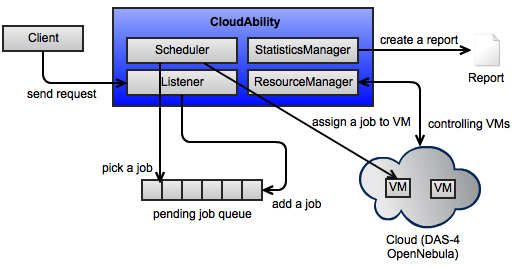
\includegraphics[width=0.35\textwidth]{pictures/system-arch.png}
\caption{CloudAbility Architecture Overview}
\label{figure_system_arch}
\end{figure}

The server part of the system consists of the following components:

\begin{enumerate}
\item\emph{Listener}:
The listener is responsible for accepting client requests through
socket connection, parsing them, and put the jobs into the pending job
queue.
\item\emph{Scheduler}:
The scheduler is the core thread in the system. It does scheduling
according to the given allocation and provisioning policies and
updates current system status. It will be explained in more details in
the later part.
\item\emph{ResourceManager}: 
This component manages the VM instances on the cloud. It also holds the
provisioning policy and provides a public interface to use it.
\item\emph{StatisticsManager} 
This module maintains all the statistics data of the system, including
job performances, VM instance performances, etc. It also generates a
final report when the system is shutting down.
\end{enumerate}

Our system is currently only runnable on \textsc{das-4} OpenNebula
platform, but it can be easily modified and extended to support other
cloud platforms. It is easy to create new allocation and provisioning
policies. All configurations are done through a configuration file.


\subsection{Resource Management Architecture}
Some features must be explained before we go to more details.

\subsubsection{Jobs}
There are three job queues in the system: \emph{pending job queue},
\emph{running job queue}, and \emph{finished job queue}. A pending job
will be picked by the scheduler and assigned to a VM instance. Then a
thread for executing this job is created, and the execution is done in
the following sequence:

\begin{enumerate}
\item Downloading required files (in our case, executable tarball and
  input files).
\item Extracting the executable tarball.
\item Executing the job (converting H.264 video file into
  \textsc{ntsc-dvd}).
\item Uploading the resulting \textsc{dvd} file to the server.
\end{enumerate}

All these operations are done through \textsc{scp} and \textsc{ssh}.
The job thread is also responsible for collecting its performance
statistics, including downloading time, execution time, uploading time,
etc. Once this job is done, it will be put into the
\emph{finished job queue} with its state set to
\statefinished. Later scheduler will remove this job and update the
statistics. If a job fails, it will also be put into the
\emph{finished job queue} but with its state set to \statefailed.
The scheduler will handle these failed jobs according to the given policy.

Although the parameters---which specifies which application to run, which
files to download, etc.---are configurable to make it able to do other
tasks, our design is not that flexible because this execution sequence
is hard coded in the program. We will consider using script files for job
execution.


\subsubsection{VM instances}
In OpenNebula, after a VM instance is created, its state becomes
\statepending, and you need to wait until it is \staterunning.
At this point, the VM instance is running, but it may not be actually
\emph{ready} because when it becomes \staterunning, it still needs some
time to boot the OS and initialize the system. Only after the system is
fully booted can the VM instance be accessed using \textsc{ssh}.

In our system, a VM instance is created asynchronously: a
thread called ``VMAgent'' is created every time the system creates a
VM instance. This thread first allocates the VM instance, and then
does the following things:

\begin{enumerate}
\item It waits until this VM instance becomes \staterunning.
\item It waits until the VM can be reached by ping.
\item It waits until the VM can be reached by \textsc{ssh}.
\end{enumerate}

After the VM is reachable, it is added into the VM list in the
ResourceManager, and it becomes available for jobs to execute on.

Each VMAgent has a timeout of two minutes. If the operation times out,
the VM instance will be terminated.

\subsubsection{Scheduler}
What the scheduler does is as follows:

\begin{enumerate}
\item It does some regular checks and updates, which will be explained
  later.
\item It picks a job from the \emph{pending queue} using the specified
  job allocation policy.
\item It picks a VM instance using the specified resource provisioning
  policy.
\item It executes this job on this VM instance.
\end{enumerate}

In the regular check part, the scheduler does miscellaneous tasks,
including:
\begin{itemize}
\item Updating job states, VM instance states, and system states.
\item Checking the \emph{finished job queue}. If a job is finished
  successfully, it is removed and its data is used to update the
  statistics. If it failed, it will be handled according to the given
  job allocation policy. For now, the system just puts a failed job into
  the \emph{pending job queue} again regardless of how many times it
  has failed.
\item Calling the provisioning policy to perform elastic provisioning.
\end{itemize}

In this way, the statistics of the system is continuously recorded,
and flexible allocation policies and elastic provisioning policies can
be implemented.


\subsubsection{Reliability}
Our system keeps track of every job and VM instance. During the
shutdown sequence, it first stops all executing jobs. Then, it
terminates all allocated VM instances, so that no VM instance would be
running afterwards. After that, it checks jobs in all the queues, and
put them into the statistics module, which finally creates a report
and outputs to a file.

Besides that, our system also keeps separate log files for the system
itself and each jobs respectively.


\subsection{System Policies}
We have implemented one job allocation policy and two resource
provisioning policies.

\subsubsection{Allocation Policy}
The job allocation policy we implemented is a First-Come-First-Serve
(\textsc{fcfs}) policy. It always picks the pending job with the
earliest arrival time.

\subsubsection{Provisioning Policies}
We implemented two provisioning policies: \policystatic{} policy and
\policysimpleelastic{} policy.

The \policystatic{} policy allocates a fixed number of VM instances when the
system starts, and this number will not vary over time. This policy
can not adapt itself to the changing environment.

The \policysimpleelastic{} policy is an on-demand-like elastic policy, which has
three parameters:

\begin{itemize}
\item \emph{min-vms}: The minimum number of VM instances the system
  must have.
\item \emph{max-vms}: The maximum number of VM instances the system can
  have.
\item \emph{threshold}: A threshold value, which will be explained
  later.
\end{itemize}

Each time the system statuses have been updated by the scheduler, this
provisioner is called and it checks the number of pending jobs. If
this number is larger than the \emph{threshold}, it creates one more
VM instance until either (1) the total number of VM instances in the
system equals the sum of pending jobs and running jobs or (2) it reaches
the \emph{maxvms}. However, when the pending job queue becomes empty,
this policy will find one idle VM instance and release it.

The \policysimpleelastic{} policy is a simple on-demand policy is because
it doesn't take into account how long a VM instance has been idle. It simply
terminates one if it is currently idle. A main drawback of this policy
can be illustrated in this example: suppose there are 7 jobs running,
no pending jobs, and 8 VMs in the system. So this policy will remove
one idle VM. If a job arrives right after the policy removes a VM,
this job has to wait for a long time to obtain an available VM.


% Section 4 - Experimental Results
\section{Experimental Results}\label{experiment}
% ========================================
% Experimental Setups Section
% ========================================
\subsection{Experimental Setups}
We carried out our experiments on DAS-4 using OpenNebula platform. The
VM image we use is CentOS-5.4 whose image ID is 35, and our VM setup
is CPU=1, VCPU=2, with 1024MB memory.

We prepared three H.264 1080p movie trailers downloaded from Apple
Trailers\footnote{http://trailers.apple.com/trailers/}, which are
described in Table \ref{table_joblist}:

\begin{table}[!t]
  \caption{Jobs for Testings}
  \label{table_joblist}
  \centering
  \begin{tabular}{|l|l|l|l|}
    \hline
    Job Name & File Name & Encoding & File Size\\
    \hline
    \texttt{job1} & cloudatlas-trailer1b\_h1080p.mov & H.264 1080p & 172MB \\
    \hline
    \texttt{job2} & skyfall-tlr2\_h1080p.mov & H.264 1080p & 180MB \\
    \hline
    \texttt{job3} & taken2-tlr1\_h1080p.mov & H.264 1080p & 175MB \\
    \hline
  \end{tabular}
\end{table}

For testing the provisioning policies, we created three different jobs
with respect to these three files. Each job is to convert a H.264
1080p video file into an NTSC-DVD file. We then randomly generated
three workloads, each of which comprises of 40 jobs. The job arrival
times are generated using exponential distribution with three
different mean interval values: 10, 20, and 30 seconds.

\begin{table}[!t]
  \caption{Workloads for Testings}
  \label{table_workloadlist}
  \centering
  \begin{tabular}{|l|l|l|}
    \hline
    Workload Name & Number of Jobs & Job Arrival Time Distribution \\
    \hline
    \texttt{wl-10} & 40 & Exponential(10) \\
    \hline
    \texttt{wl-20} & 40 & Exponential(20) \\
    \hline
    \texttt{wl-30} & 40 & Exponential(30) \\
    \hline
  \end{tabular}
\end{table}


% ========================================
% Experiments
% ========================================
\subsection{Experiments}

% ========================================
% Benchmark Tests
% ========================================
\subsubsection{Benchmark Tests}
First, we did four benchmark tests to measure the performance of DAS-4
OpenNebula:

\begin{enumerate}
\item The first three tests run the three jobs separately. Each
  test is done 20 times, and we measure the job's running times
  (the total amount of time a job spent on its execution).
\item In another test, we continuously allocate and release a VM
  instance for 20 times in order to measure the overhead of allocating
  a VM instance on DAS-4.
\end{enumerate}

\begin{figure}[!t]
\centering
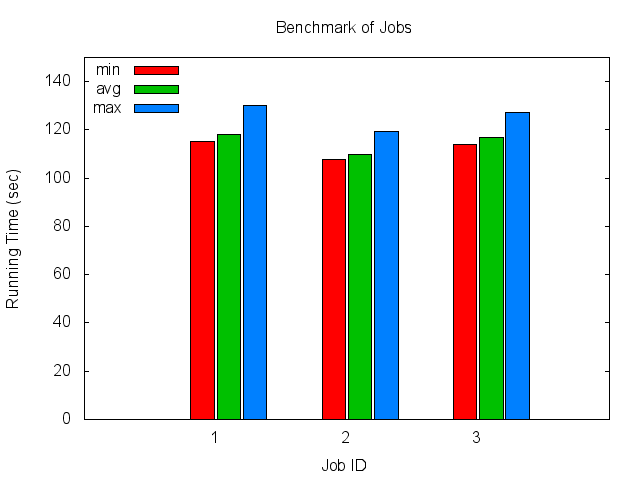
\includegraphics[width=0.35\textwidth]{pictures/benchmark-jobs.png}
\caption{Results of the benchmark tests for jobs}
\label{figure_jobbenchmark}
\end{figure}

As illustrated in Fig. \ref{figure_jobbenchmark}, all three jobs takes
almost the same amount of time to finish, with an average of 114.819 seconds, and there is no huge deviation from the average.

\begin{figure}
\centering
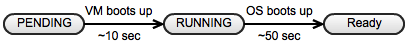
\includegraphics[width=0.35\textwidth]{pictures/vm-preparation-model.png}
\caption{VM Preparation Model}
\label{figure_vm_preparation_model}
\end{figure}

Figure \ref{figure_vm_preparation_model} is the model that we use to analyze
the VM allocation overhead. We measured the total preparation time of a VM,
which is the time from it is allocated until it is accessible through
\textsc{SSH}. The allocation time is from the VM instance is
allocated until its state becomes \staterunning, and the OS booting time is
the time after that and until this VM is accessible through \textsc{SSH}.

\begin{table}
\caption{Total Preparation Time of VMs}
\label{table_vm_preparation}
\centering
\begin{tabular}{|l|l|}
\hline
Average Total Preparation Time & 60.309 seconds \\
\hline
Average Allocation Time & $\approx$10 seconds \\
\hline
Average OS Booting Time & $\approx$50 seconds \\
\hline
\end{tabular}
\end{table}

Table \ref{table_vm_preparation} shows the results of our the VM allocation
overhead test. We only put the average values here because the minimum and
maximum values are close. The results suggest that the DAS-4 OpenNebula
is efficient in allocating a VM instance. It only takes approximately 10
seconds to become RUNNING after it is allocated. However, it takes
approximately 50 seconds for a VM to boot up its OS, which becomes the major
overhead of allocating a new VM.


% ========================================
% Experiments on the Provisioning Policies
% ========================================
\newcommand{\STATIC}{\textsc{static}}
\newcommand{\SE}{\textsc{se}}
\newcommand{\SEzero}{\textsc{se-0}}
\newcommand{\SEfive}{\textsc{se-5}}

\subsection{Experiments on the Provisioning Policies}
In this part, we use the three workloads to test the two policies. We
use three settings here:
\begin{enumerate}
\item \policystatic{} with 5 VMs. We call this \STATIC{} for short.
\item \policysimpleelastic{} that has 5 to 20 VMs, with \emph{threshold} set to 0. We call this \SEzero{} for short.
\item \policysimpleelastic{} that has 5 to 20 VMs, with \emph{threshold} set to 5. We call this \SEfive{} for short.
\end{enumerate}

\begin{figure}[!t]
\centering
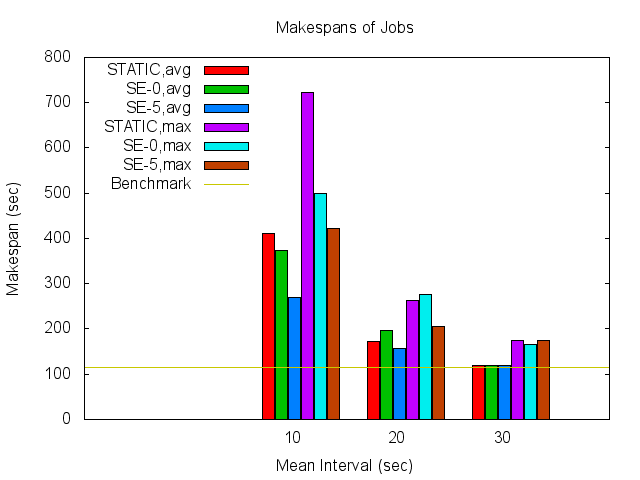
\includegraphics[width=0.35\textwidth]{pictures/all-makespans.png}
\caption{Makespans of jobs in the three workloads}
\label{figure_jobmakespan}
\end{figure}

Figure \ref{figure_jobmakespan} illustrates the job makespans of different
policies in each workload. The brown line indicates the average running time
of a job is the benchmark test. As expected, for \texttt{wl-10},
\SE{} outperforms the \STATIC{} both in the average case
and the worst case. \SEfive{} achieves the best job makespan for both
\texttt{wl-10} and \texttt{wl-20}. For \texttt{wl-30}, the performances are
almost the same, which suggests that five VMs are enough for \texttt{wl-30}.

Another observation is that, for \texttt{wl-10} and \texttt{wl-20}, the
average job makespans are both higher than the benchmark result. In another
test which we allocated 30 VMs, we find that there are totally 8 nodes being
used, each of which has 4 VMs or so on it. Also, comparing the detailed
job execution results (not present here), we find that DAS-4 OpenNebula's
over-allocation has a great impact on the VM performance. Computation, I/O
and network performances can all be influenced.

\begin{figure}[!t]
\centering
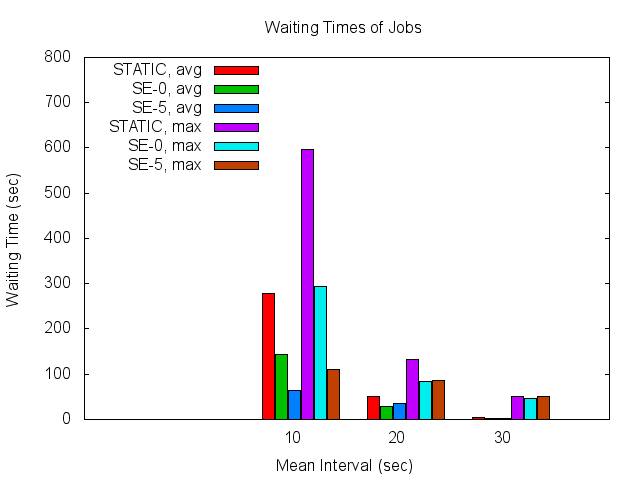
\includegraphics[width=0.35\textwidth]{pictures/all-waittimes.png}
\caption{Waiting times of jobs in the three workloads}
\label{figure_jobwaittime}
\end{figure}

For \texttt{wl-20}, Fig. \ref{figure_jobwaittime} shows that \SEzero{} has
the lowest job waiting time, however from \ref{figure_jobmakespan}, we
see that the job makespans are the highest. We believe that this slowdown
may be caused by DAS-4 OpenNebula's over-allocation of VMs. According to
our statistics, this slowdown can be 3.64 at max and 1.91 in average in
\textsc{wl-10}.

\begin{figure}[!t]
\centering
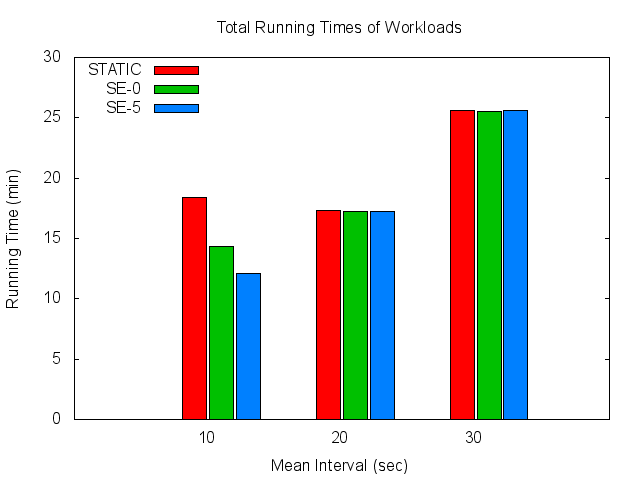
\includegraphics[width=0.35\textwidth]{pictures/workload-runtime.png}
\caption{Total makespan of three workloads}
\label{figure_workloadmakespan}
\end{figure}

The total makespans of each workload, which is depicted in Fig.
\ref{figure_workloadmakespan}, also suggests that \SE{}
achieves much better performance than \STATIC{} for \texttt{wl-10}.


% ========================================
% VM Performance Section
% ========================================
\subsection{VM Performances}\label{section_vm_performance}
We analyze the utilization of VMs in our system in this part. The
utilization level is the fraction of time VMs spent on running jobs
with respect to their total lifetime, and it can be described by
Equation \ref{equation_vm_util}.

\begin{equation}
\label{equation_vm_util}
Utilization = \frac{\sum{T_{running\_jobs}}}{\sum{T_{lifetime}}}
\end{equation}

\begin{figure}[!t]
\centering
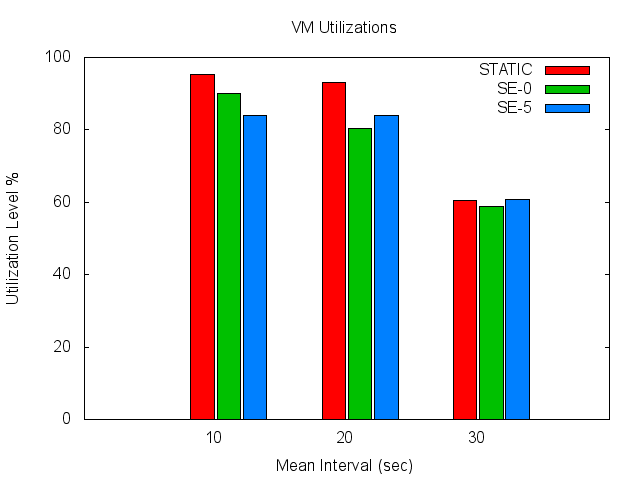
\includegraphics[width=0.35\textwidth]{pictures/vm-util.png}
\caption{VM Utilizations Levels}
\label{figure_vm_util}
\end{figure}

The results are illustrated in Fig. \ref{figure_vm_util}. Although in
\texttt{wl-10} and \texttt{wl-20}, the utilization levels of \SE{} are
lower than \STATIC{}, the decrements are acceptable. \SE{} can utilize
the VMs relatively efficiently.

Due to \SE{}'s feature that it terminates an idle VM as soon as there is
no pending jobs, we would also like to analyze its drawback.
For doing this, we measure the number of wasted VMs by using \SE{}.
A \emph{wasted VM} is a VM that has not got any job running on it during
its whole lifetime.

A VM can be wasted in this scenario: suppose we are using \SEzero{},
and there are 5 VMs in the system with 5 jobs running on them
respectively. Then a new job comes, and \SEzero{} will allocate a new VM,
say $VM_{new}$. However, before $VM_{new}$ becomes available, one
running job has been finished, which means a VM becomes idle, and this
new job is then assigned to this free VM. So, when $VM_{new}$ is
ready, the pending job queue is empty, and according to our policy,
$VM_{new}$ is terminated. In this case, no job has been running on
$VM_{new}$ during its lifetime, and we say that $VM_{new}$ is wasted.

In Fig. \ref{figure_vm_wasted}, we can see that in \texttt{wl-10},
the number of \SEzero is as high as 23, while \SEfive has no wasted VM
at all. \SEfive also has a low number of wasted VMs in the other two cases,
no exceeding 3.

\begin{figure}[!t]
\centering
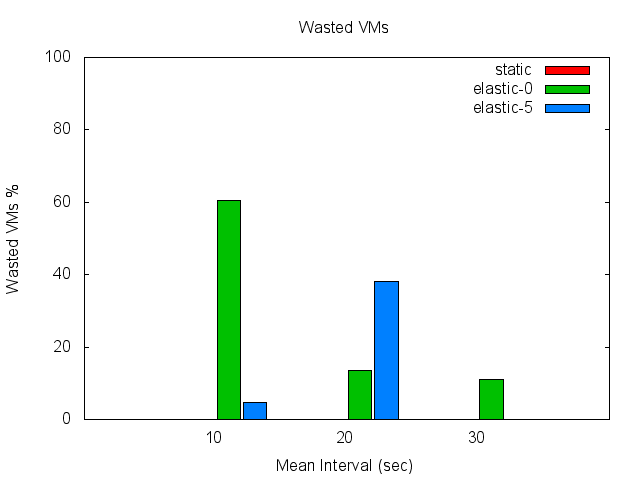
\includegraphics[width=0.35\textwidth]{pictures/vm-wasted.png}
\caption{Wasted VMs}
\label{figure_vm_wasted}
\end{figure}


% ========================================
% Speedup vs. Cost Tradeoff Section
% ========================================
\subsection{Speedup vs. Cost Tradeoff}
In this part, we calculate the speedups of using our SE provisioning
policy and the charged-costs. Because our VM setup has no
corresponding machine on Amazon Web Service, we use the charged cost
of m1.medium (\$0.16 per hour for Linux), which has two compute units,
for our charged-cost calculation. Table \ref{table_chargedcosts} shows
the results.

\begin{table}
\caption{Charged-costs}
\label{table_chargedcosts}
\centering
\begin{tabular}{|l|l|l|l|}
\hline
Workload & STATIC & SE-0 & SE-5 \\
\hline
\texttt{wl-10} & 1.54hrs (\$0.246) & 2.86hrs (\$0.458) & 2.73hrs (\$0.437) \\
workspan (min)&18.43 &14.36 &12.09\\
\cline{2-4}
&\multicolumn{3}{|c|}{extrapolated with workspan runtime}\\
\cline{2-4}
&1d  (\$19.22 )&1d (\$45.93)&1d (\$52.05)\\
&1m (\$576.63)&1m (\$1377.83)&1m (\$1561,48)\\
&1y (\$7015.60)&1y (\$16763.56)&1y (\$18998.11)\\
\hline
\texttt{wl-20} & 1.44hrs (\$0.230) & 2.32hrs (\$0.371) & 1.62hrs (\$0.259) \\
workspan (min)& 17.31&17.24 &17.24\\
\cline{2-4}
&\multicolumn{3}{|c|}{extrapolated with workspan runtime}\\
\cline{2-4}
&1d (\$19.13)&1d (\$30.99)&1d (\$21.63)\\
&1m (\$574.00)&1m (\$929.65)&1m (\$649.00)\\
&1y (\$6983.71)&1y (\$11310.76)&1y (\$7896.19)\\
\hline
\texttt{wl-30} & 2.13hrs (\$0.341) & 2.18hrs (\$0.349) & 2.13hrs (\$0.341) \\
workspan (min)&25.59 &25.55 &25.57\\

\cline{2-4}
&\multicolumn{3}{|c|}{extrapolated with workspan runtime}\\
\cline{2-4}

&1d (\$19.19)&1d (\$19.67)&1d (\$19.20)\\
&1m (\$575.66)&1m (\$590.09)&1m (\$576.11)\\
&1y (\$7003.89)&1y (\$7179.4)&1y (\$7009.37)\\

\hline
\end{tabular}
\end{table}

\begin{table}
\caption{Speedups and Costs for wl-10}
\label{table_speedupcost}
\centering
\begin{tabular}{c|c|c|c|c|}
\cline{2-5}
 & \multicolumn{2}{c|}{\texttt{wl-10}} & \multicolumn{2}{c|}{\texttt{wl-20}} \\
\cline{2-5}
 & \SEzero & \textbf{\SEfive} & \SEzero & \textbf{\SEfive} \\
\hline
\multicolumn{1}{|c|}{Speedup} & 1.28 & \textbf{1.52} & 1.00 & \textbf{1.00} \\
\hline
\multicolumn{1}{|c|}{Cost} & 1.86 & \textbf{1.78} & 1.61 & \textbf{1.13} \\
\hline
\end{tabular}
\end{table}

We mainly focus on the results of \texttt{wl-10}, because this is the
only case that \SE outperforms \STATIC. From Table
\ref{table_speedupcost}, we can see that only \SEfive is close to
cost-speed proportional in both \texttt{wl-10} and \texttt{wl-20}.
The results suggest that it is not an easy task to achieve
cost-efficiency even in a simple cloud system.

If we extrapolate the numbers we get the numbers in Table
\ref{table_chargedcosts}. The numbers have been calculated by taking
the costs of the workloads extrapolated over their workspan time,
i.e. the costs which would have incurred if the tests were run
repeatedly for the designated extrapolated time period.



% Section 5 - Experimental Results
\section{Discussion}\label{discussion}

%%main findings summary

\subsection{Findings}
In this section we will discuss the findings of the experiment.

\paragraph{Makespan}
In Fig.~\ref{figure_jobmakespan} we can see that the static allocation
has the highest makespan, the rationale behind this, is that during
the peak usage in the sample workload, there will be jobs that will
have to wait a relatively long time due to the static nature of the
policy and due to the almost equally sized jobs and
\textsc{fcfs}-policy - the job which is added when the queue is largest
will also have the largest makespan.

%% tradeoffs -- added by Lipu Fei, please check
The tradeoff table \ref{table_speedupcost} shows that our
\policysimpleelastic{} policy achieves a better speedup-cost tradeoff
with its \emph{threshold} set to 5. However, our workloads for testing
are relatively simple, so it could get worse when the system is more
overloaded.


%% drawbacks of SimpleElastic provisioning (VM waste)
%% -- added by Lipu Fei, please check

What is interesting to see is that the SE-0 has higher makespan for
the 20ms mean interval, but not for the 10ms and 30ms mean interval
but can be explained as mentioned in \ref{section_vm_performance} --
an obvious drawback of our \policysimpleelastic{} provisioning policy
is that it can waste allocated VMs.  Especially for \SEzero{}, in the
workload \textsc{wl-10} it has a significant overhead. This is mainly
caused by the immediate termination of VMs when no pending job
available. A improvement can be made by adding an \emph{aggregate idle
  time}, indicating how long a VM has been idle since (1) it was
created or (2) the last time it finished a job, and also setting up a
new threshold. When the pending job queue is empty, the provisioning
policy updates all VMs' \emph{aggregate idle time} and terminates a VM
with its \emph{aggregate idle time} higher than the threshold.  A more
structural improvement would be to see if the boot time of the VM's OS
can be shortened. This would probably positively influence the results
a lot, however making such adjustments to the provided IaaS in
question -- OpenNebula on \textsc{das-4} -- is not trivial due to
lacking permissions for such adjustments. However we could test with
artificial boot-times by allocating the maximum amount of VMs in
advance and then imitate the availability of the VMs after the desired
amount of time we'd like to test. That way we can see how much there
is to gain by making the boot sequence more efficient. Also the
pausing and resuming of VMs could be implemented which could cause for
a more simple implementation.

%% Some other discussions
%% -- added by Lipu Fei, please check
Besides the above, in reality, the video conversion jobs submitted by
users are probably larger files sizing more than 4GB, which is the
conventional size of a \textsc{h.264} movie. If the time it takes for
a video to convert goes linearly with the size of the input file, then
a 4GB will probably take more than 40 minutes to finish with our
current VM setup. An enhancement to this would be to create a
decentralized system that works in the this way: when a job arrives,
the system assigns it to a VM. The VM first checks the size of the
input, and it divides the input file into two (or more) equal-sized
parts if the original size is too large.  The smaller parts are then
sent to other VMs, who process the input in the same way. When the
size is small enough, a VM will convert the input. This VM can be
considered a leaf node in the tree of VMs. All parent nodes will wait
for their child nodes to finish and upload the results, and then merge
them in order. Finally, the root node will get all the merged
result. We think this is doable, for \textsc{FFmpeg} is very efficient
in concatenating two video files. Through this method not only would
our application scale in the number of jobs, but also scale in the
size of individual jobs.

%% about future work, may be put into another paragraph
%% -- added by Lipu Fei, please check
So for future work, we are considering the following options:
\begin{enumerate}
\item Carrying out a benchmark test on larger input files to get the
  growth of job's running time against input size.

\item Improving the current provisioning policy with our proposed
  suggestion using threshold after which VMs can be released.
\item Improving boot times through more efficient OS boot-time and/or
  make use of pausing/resuming VMs.

\item Create a decentralize system that uses divide-and-conquer
  mechanism to solve large inputs.

\end{enumerate}



%%recommendation

%% extrapolation


% Section 6 - Experimental Results
\section{Conclusion}\label{conclusion}
This is conclusion section.

% Appendix A - Time Sheets
\appendix[Time Sheets]
\begin{table}
  \caption{Time Sheet Table for the Whole Lab Exercise}
  \centering
  \begin{tabular}{l|l}
    \hline
    Parts       & Time \\
    \hline
    total-time  & \\
    think-time  & \\
    dev-time    & \\
    xp-time     & \\
    write-time  & \\
    wasted-time & \\
    \hline
  \end{tabular}
\end{table}

% Bibliographies
\bibliographystyle{IEEEtran}
\bibliography{Report.bib}
\end{document}
